\documentclass[9pt, apectratio=43,unicode]{beamer}
\usetheme{Moscow}

\usepackage[utf8]{inputenc}
\usepackage[T2A]{fontenc}
\usepackage[main=russian,english]{babel}

\usepackage{amsmath,amssymb}

\renewcommand{\thefootnote}{\fnsymbol{footnote}}
\hypersetup{pdfauthor={Paul Ostanin}}

%\usepackage{concmath}
%\usepackage{euler}

\usepackage{mathtools}

\graphicspath{ {images/} }

\title[Моделирование F слоя Земной ионосферы]{Моделирование F слоя Земной ионосферы}
\author[Останин П. А.]{Останин Павел Антонович  \\ \vspace{1ex} Научный руководитель: Кулямин Дмитрий Вячеславович}

\date{ }
\newcommand{\colorhref}[2]{\href{#1}{\textcolor{miptbase!30!black}{#2}}}

\begin{document}

\begin{frame}[plain]
\titlepage
\end{frame}

\def\L{\mathcal{L}}

\section{Постановка задачи}
\begin{frame}\frametitle{Задачи и актуальность}
\begin{itemize}
\item[•] Разработка динамической трёхмерной модели F слоя ионосферы;
\item[•] Разработка совместной модели термосферы-ионосферы со включением модели ионосферы как вычислительного блока.
\end{itemize}

Актуальность проблемы и её прикладное значение:
\begin{itemize}
\item[•] Задачи космической отрасли;
\item[•] Межконтинентальная и спутниковая радиокоммуникация;
\item[•] Радиолокация и навигационные системы: состояние ионосферы определяет характеристики движения низкоорбитальных спутников;
\end{itemize}


\end{frame}

\begin{frame}\frametitle{Используемые приближения; векторное уравнение}

Используемые приближения:
\begin{itemize}
\item[•] Рассмотрение только F слоя; Динамическое преобладание амбиполярной диффузии;
\item[•] Предположение квазинейтральности плазмы;
\item[•] Одноионная постановка с рассмотрением иона $O^+$;
\item[•] Дипольное приближение магнитного поля Земли;
\end{itemize}

Уравнение, описывающее эволюцию электронной концентрации (уравнение неразрывности): $$\dfrac{\partial n_i}{\partial t} = -div(n_i \vec{u}_\parallel)-div\left(n_i\dfrac{1}{B^2}[\vec{E}\times \vec{B}] \right)+$$ $$+div\left(D\left[\nabla_\parallel n_i +n_i\dfrac{1}{T_p}\nabla_\parallel T_p - \dfrac{n_i m_i}{2kT_p}\vec{g}_\parallel\right]\right)+[P-k_in_i].$$

\end{frame}

\begin{frame}\frametitle{Уравнение в сферической системе координат (в приближении тонкого сферического слоя)}

$$\dfrac{\partial n_i}{\partial t} = DYZ(n_i)+DTr(n_i)+[P-kn_i].$$

$$DYZ(n_i) = \dfrac{1}{a\cos\varphi}\dfrac{\partial}{\partial\varphi}\left(D\cos\varphi\left[\dfrac{1}{a}\dfrac{\partial n_i}{\partial\varphi} \cos^2 I -\dfrac{\partial n_i}{\partial z}\cos I\sin I\right]\right)+ \dfrac{\partial}{\partial z}\bigg(D\bigg[\dfrac{\partial n_i}{\partial z}\sin^2 I -$$ $$- +Tr(n_i)+Tr(n_i)\dfrac{1}{a}\dfrac{\partial n_i}{\partial\varphi}\cos I \sin I\bigg]\bigg);$$ 

$$DTr(n_i) = \dfrac{1}{a\cos\varphi}\dfrac{\partial}{\partial \varphi}\bigg[\bigg(\dfrac{1}{a}\dfrac{1}{T_p}\dfrac{\partial T_p}{\partial\varphi}\cos^2 I-\dfrac{1}{T_p}\dfrac{\partial T_p}{\partial z}\cos I \sin I - \dfrac{1}{H}\sin I \cos I\bigg)Dn_i\cos\varphi\bigg] +$$ $$+ \dfrac{\partial}{\partial z}\bigg[\bigg(-\dfrac{1}{a}\dfrac{1}{T_p}\dfrac{\partial T_p}{\partial \varphi}\cos I \sin I +\dfrac{1}{T_p}\dfrac{\partial T_p}{\partial z}\sin^2 I+\dfrac{1}{H}\sin^2I\bigg)Dn_i\bigg].$$
%\end{frame}

%\begin{frame}\frametitle{Upper boundary condition}

На верхней границе ставится условие третьего рода, в котором полный поток считается известным и близким к нулю:
$$D\left(\dfrac{\partial n}{\partial z} \sin^2 I - \dfrac{1}{a}\dfrac{\partial n}{\partial \varphi} \cos I \sin I + \dfrac{1}{H} n \cdot \sin^2 I\right) = F_{ub} \approx 0.$$
\end{frame}

\begin{frame}\frametitle{Особенности системы уравнений модели ионосферы}

Постановка уравнения содержит ряд особенностей:
\begin{itemize}
\item[•] Уравнение отражает баланс массы;
\item[•] Задача имеет геометрические особенности;
\item[•] Характерные значения коэффициента диффузии меняются экспоненциально с высотой на $6$ порядков;
\item[•] Характерные времена плазмохимических процессов малы; вместе с предыдущим пунктом это обуславливает существенную жёсткость задачи;
\item[•] Решение уравнения в силу физического смысла неотрицательно;
\end{itemize}

Симметричная матрица эффективных коэффициентов диффузии $S = \begin{pmatrix}K_1^2 & K_1K_2 \\
K_1K_2 & K_2^2 \end{pmatrix}$, где $K_1 = \sqrt{D}\cos I$, $K_2 = \sqrt{D}\sin I$, вырождена в каждой точке. 

При нулевых $P$, $k_i$ и краевых условиях интегрирование по всей области даёт соотношение: 
$$\dfrac{1}{2}\dfrac{\partial}{\partial t} \iint_{\varphi, z} (n_i)^2 \cos\varphi d\varphi dz = - \iint_{\varphi, z}\left(K_1 \dfrac{\partial n_i}{\partial\varphi} + K_2\dfrac{\partial n_i}{\partial z}\right)^2 \cos \varphi d\varphi dz \leq 0.$$

\end{frame}


\section{Численное моделирование: два подхода}

\subsection{Пространственная аппроксимация}

\begin{frame}\frametitle{Пространственная аппроксимация}
\begin{itemize}
\item[•] Для диффузионных компонент используется стандартная консервативная аппроксимация с помощью центральных разностей:

$$\dfrac{\partial}{\partial z}D\dfrac{\partial n}{\partial z} \approx \dfrac{1}{h_{i+1/2}}\left(\dfrac{D_{i+1/2}(n_{i+1}-n_i)}{h_i}-\dfrac{D_{i-1/2}(n_{i}-n_{i-1})}{h_{i-1}}\right);$$

\item[•] Гиперболические слагаемые также аппроксимированы центральными разностями;


\parbox[b][5cm][t]{50mm}{
\item[•] Ключевая особенность: наличие смешанных производных. Используется аппроксимация второго порядка, зависящая от знака $\sin I$;

{\small\textit{При постоянных коэффициентах аппроксимация удовлетворяет конечно-разностному аналогу интегрального соотношения.}}

\item[•] Верхнее граничное условие аппроксимировано в соответствии с конечно-разностными формулами для смешанных производных.
}
\hfill
\parbox[b][5cm][t]{60mm}{
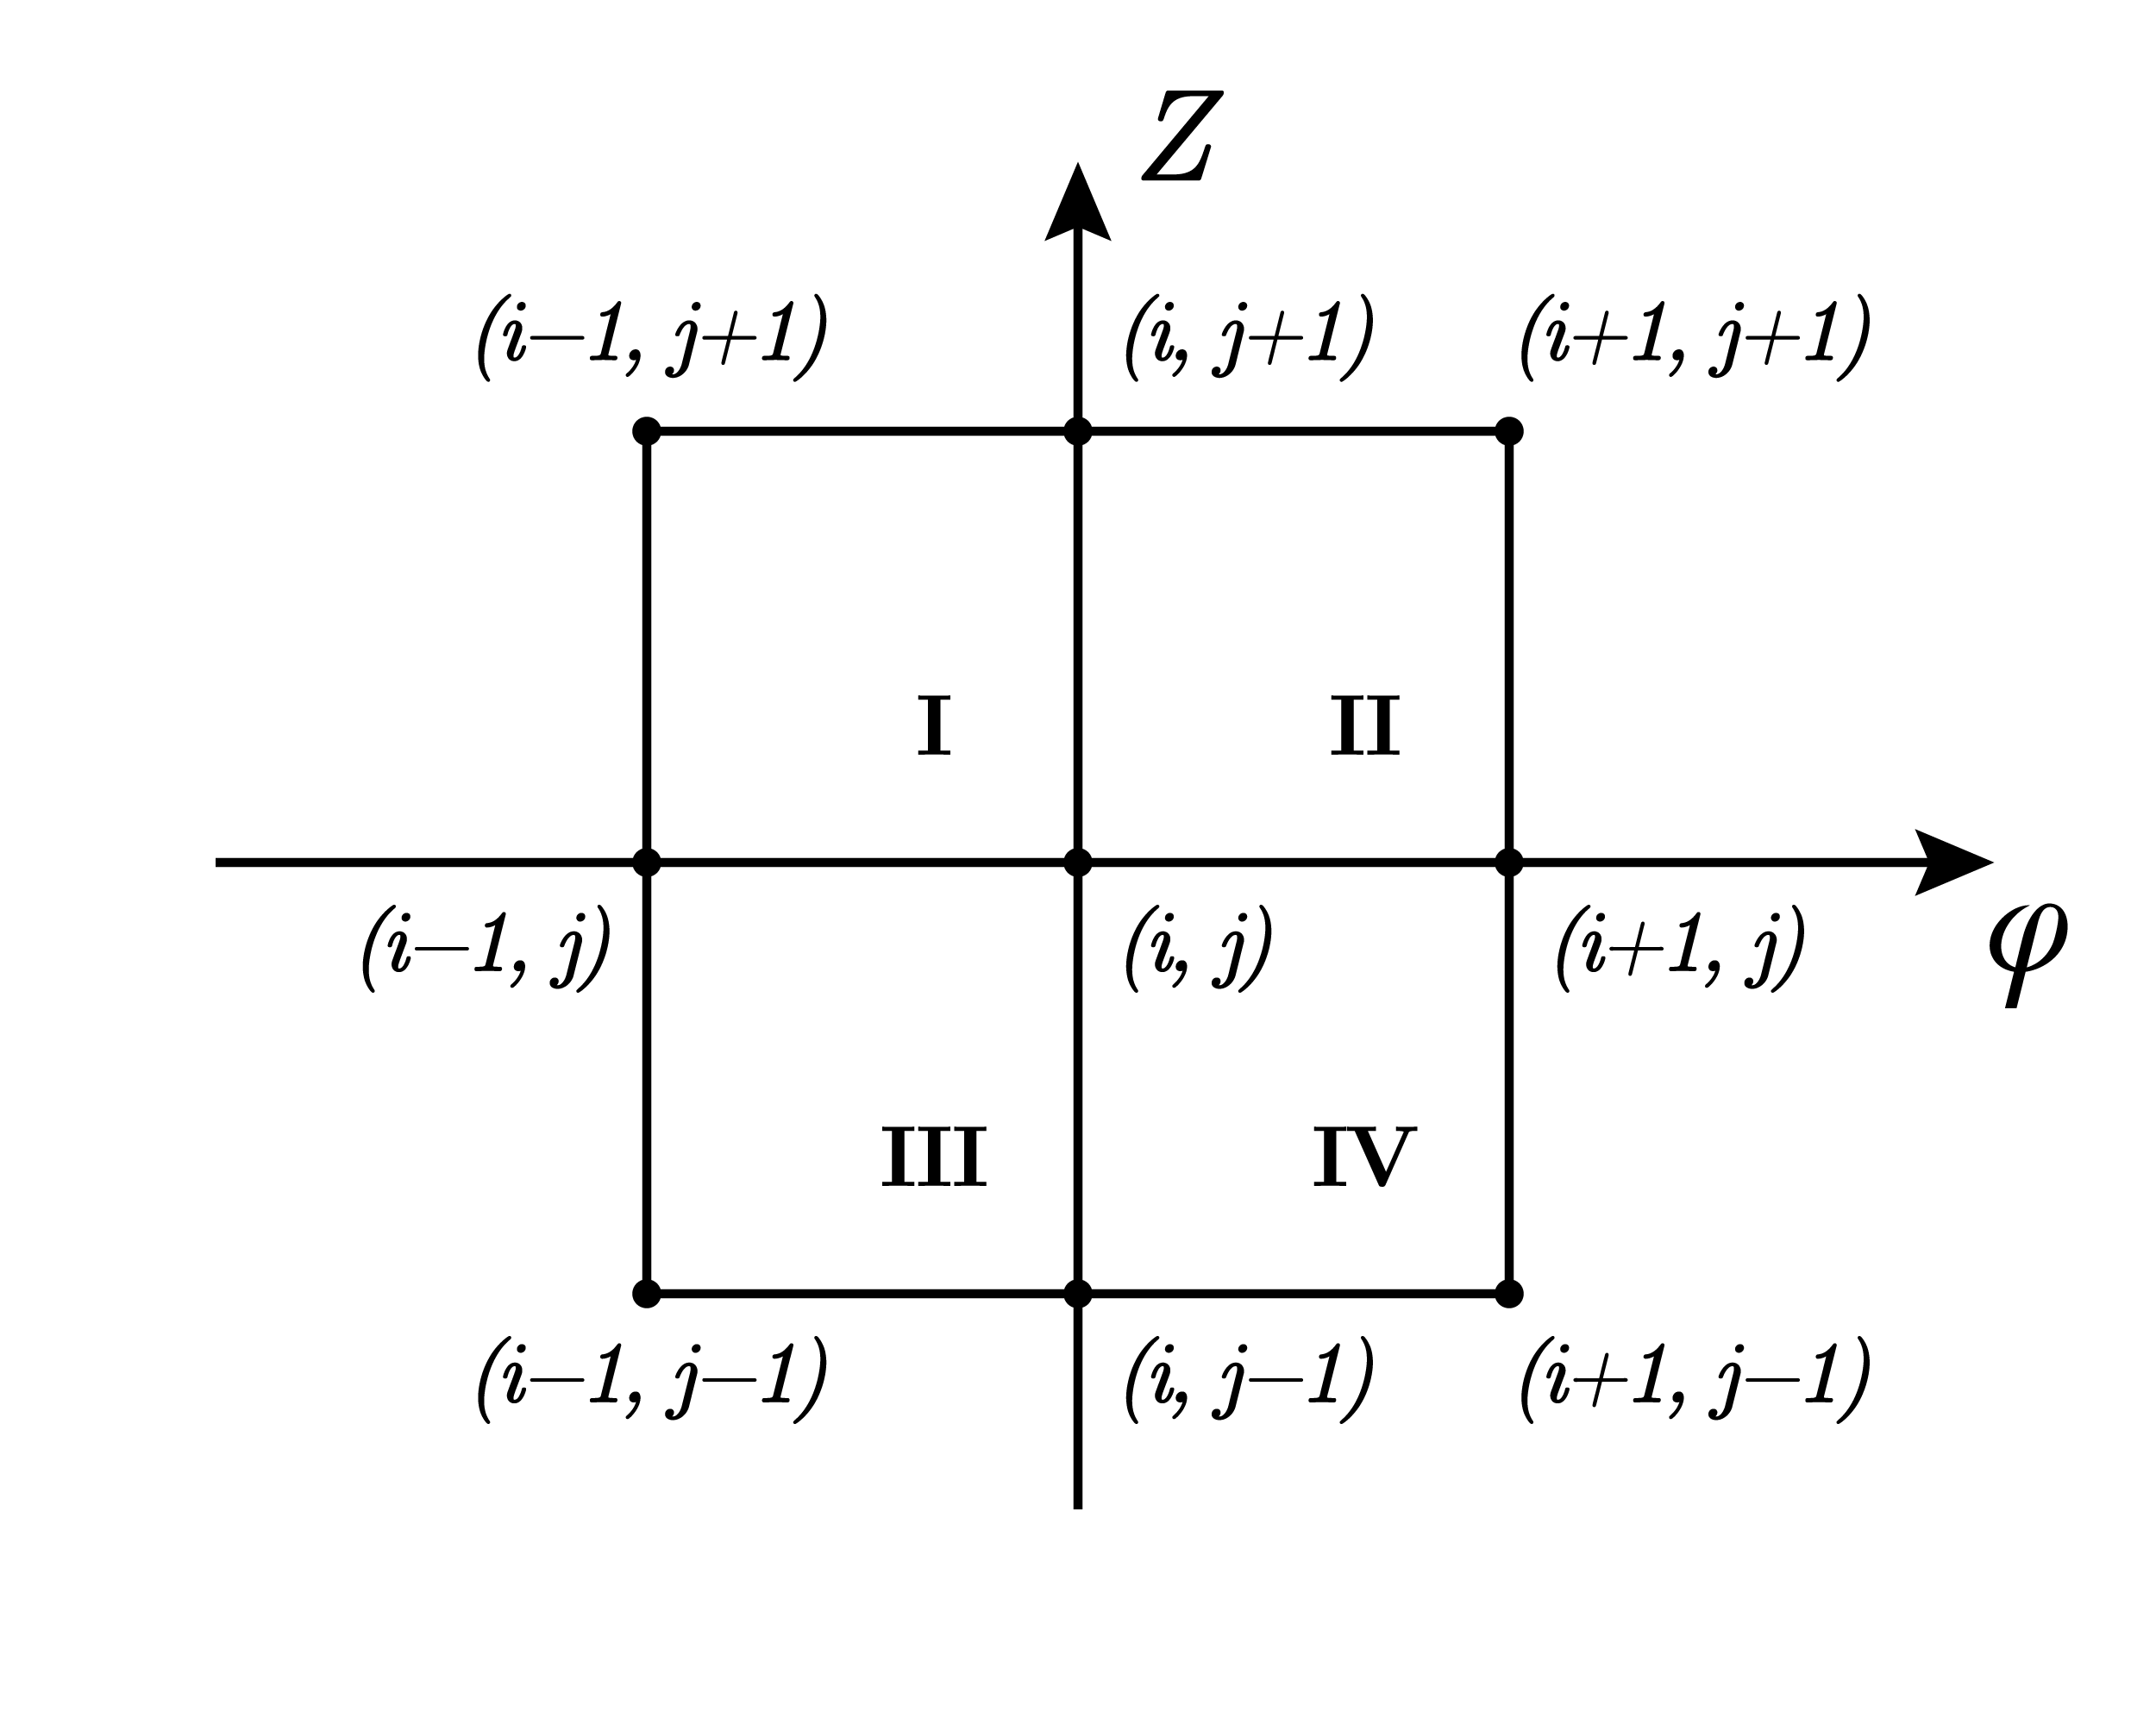
\includegraphics[scale = 0.3]{square}
}

\end{itemize}

\end{frame}


\subsection{Два способа аппроксимации по времени}
\begin{frame}\frametitle{Два способа аппроксимации по времени}

В работе сравниваются два подхода к аппроксимации по времени:

\begin{itemize}

\item[I.] Полностью неявная схема (линейная система решается с помощью метода BiCG);

\item[II.] Схема расщепления: 

\end{itemize}

\begin{itemize}

\item[•] Диффузия вдоль оси $z$, смешанные производные и фотохимия~---~первый шаг расщепления; 

\item[•] Диффузия вдоль широты~---~второй шаг расщепления;

\item[] (линейные системы на обоих шагах расщепления решаются одномерными прогонками);

\end{itemize} 



\bigskip 

\parbox[b][5cm][t]{50mm}{
Свойства схем протестированы на модельном стационарном решении: $$n_{mod}(z, \varphi) = A\cdot e^{-B(z-C)}\cdot(z-C)\cos^2\dfrac{\varphi}{2}$$ Форсинг выбран так, чтобы данная функция являлась точным решением.}
\hfill
\parbox[b][5cm][t]{60mm}{
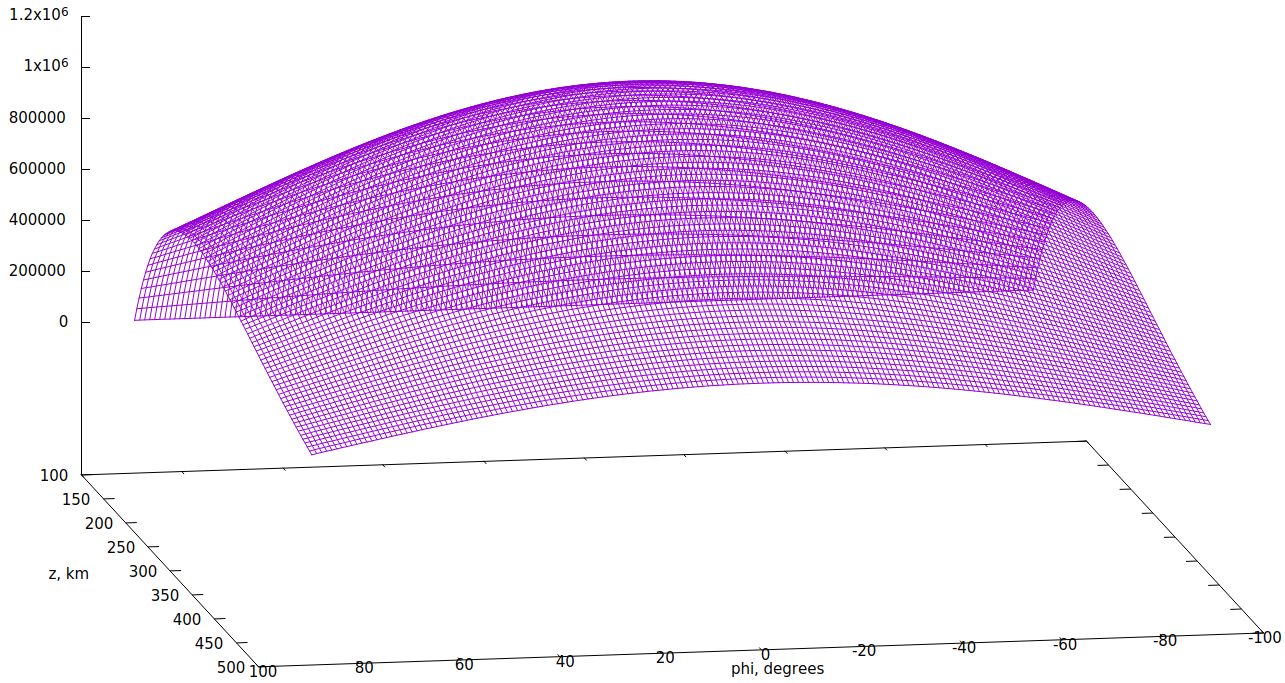
\includegraphics[scale = 0.13]{model}\\Рис. 1. Модельное решение $n_{mod}(z, \varphi)$, $z$ меняется от $100$ км до $500$ км и $\varphi$ от $-90^\circ$ до $90^\circ$.
}
\end{frame}


\subsection{Сравнение аппроксимаций по времени}
\begin{frame}\frametitle{Сравнение аппроксимаций по времени}
I. Неявная схема даёт лучшую точность при больших шагах по времени;

\center{
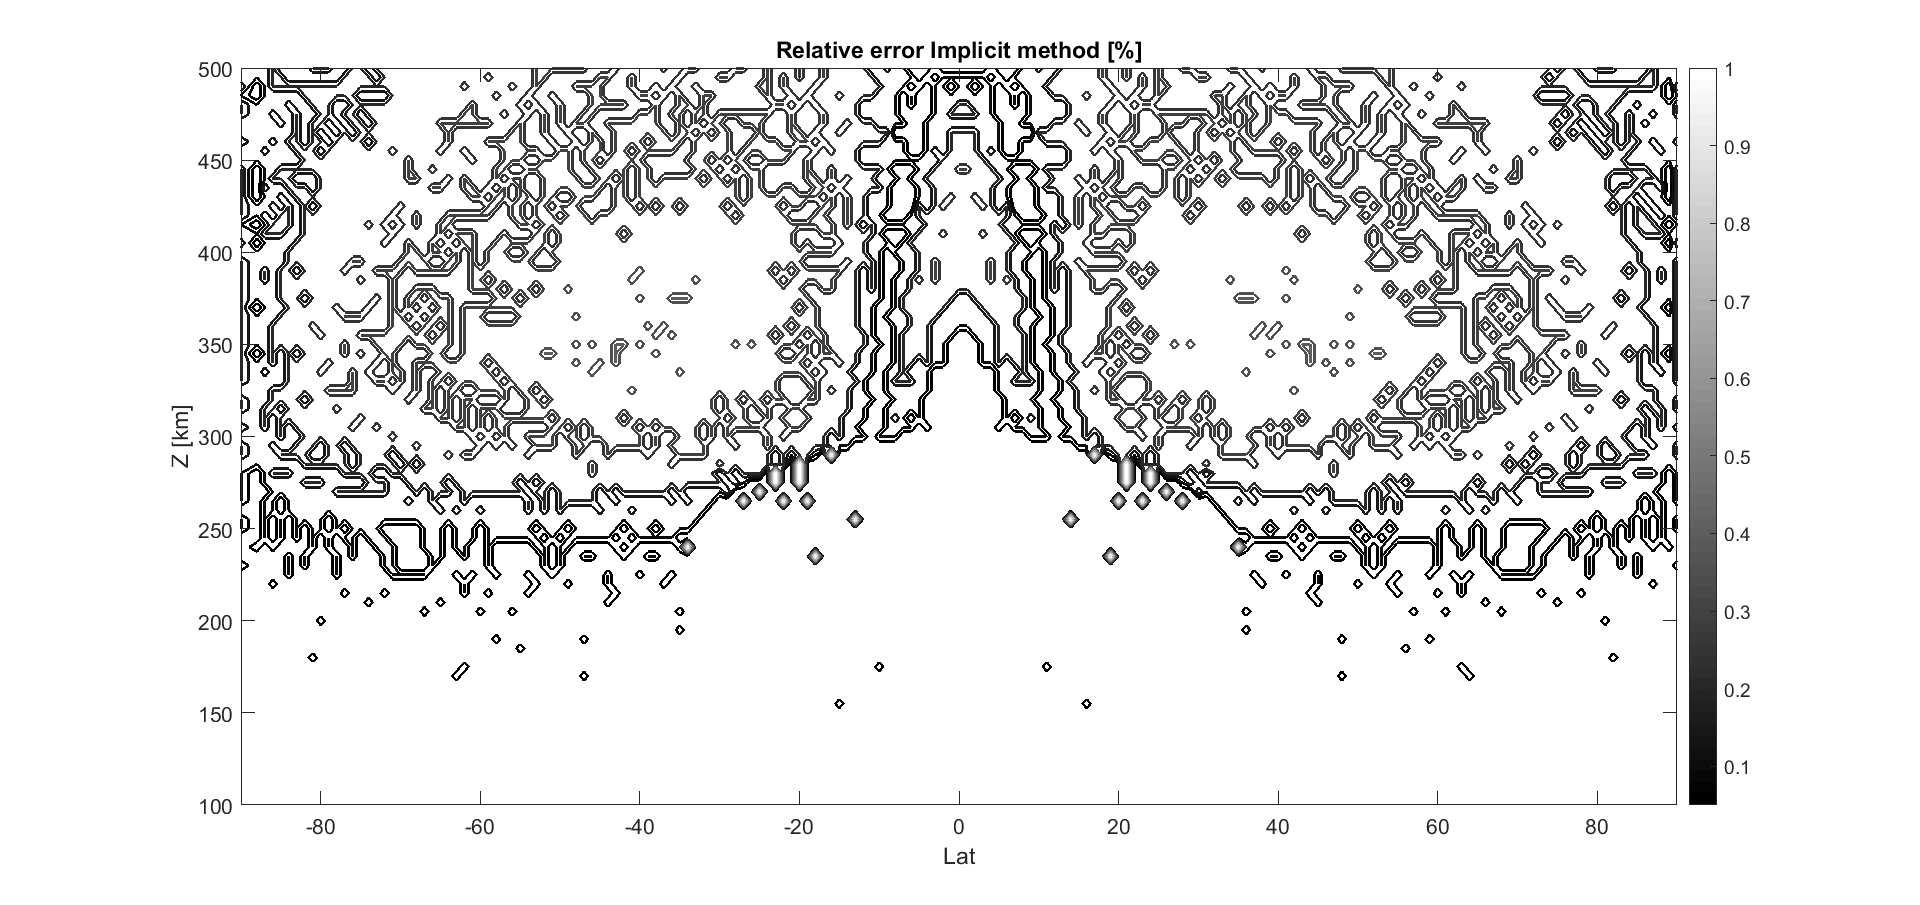
\includegraphics[scale=0.2]{diff_implicit} \\Рис. 2. Ошибка в вычислении стационарного состояния для полностью неявной схемы в задаче с заданным модельным решением.
}
\end{frame}

\begin{frame}\frametitle{Сравнение аппроксимаций по времени}
II. При заданном шаге по времени решение по методу расщепления приблизительно в $4$ раза быстрее, но дополнительная ошибка вносит существенный вклад;

\begin{center}
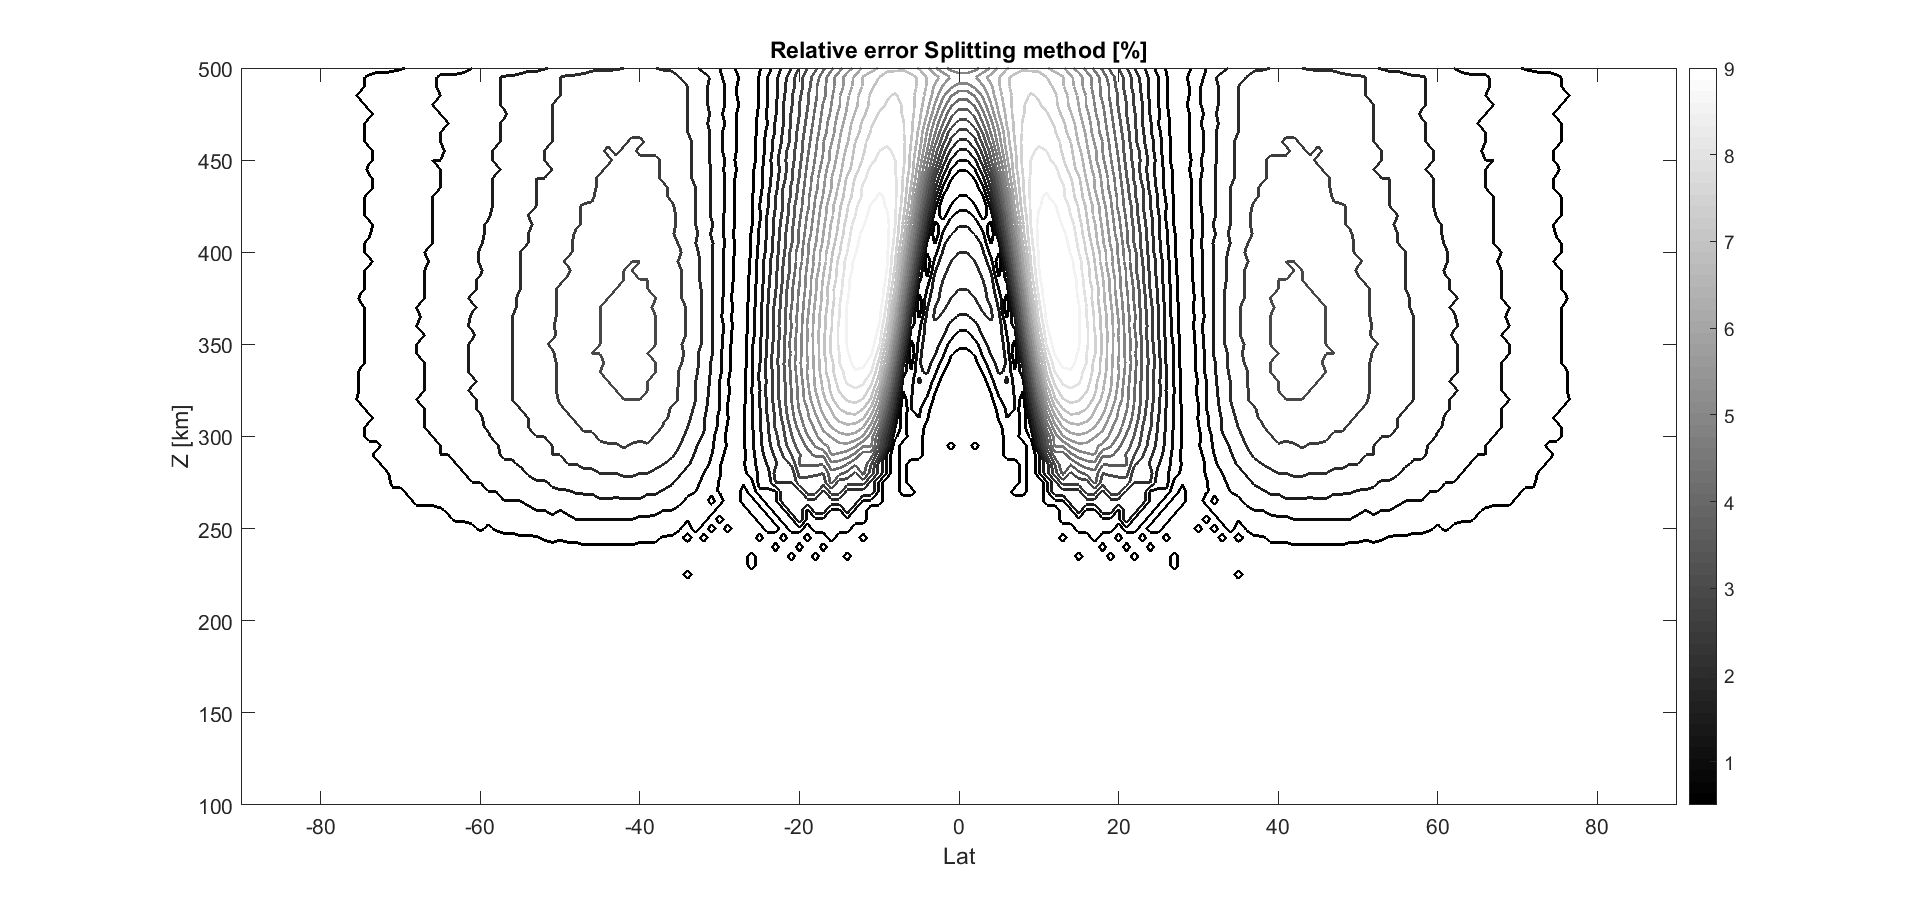
\includegraphics[scale=0.18]{splitted_tau_100}\\Рис. 3. Ошибка в вычислении стационарного состояния для метода расщепления при шаге по времени $\tau = 100$~с.
\end{center}
\end{frame}

\begin{frame}\frametitle{Заключение}
\begin{itemize}
\item[I.] Разработана первая версия двумерной динамической модели F слоя ионосферы ИВМ РАН на основе решения уравнений динамики плазмы в приближении амбиполярной диффузии в сферических геомагнитных координатах, сформулированы основные уравнения модели и предложен алгоритм поэтапной реализации на основе метода расщепления по физическим процессам;
\item[II.] Реализованы два метода численного интегрирования модели, проведено сравнение точности разработанных методов на основе аналитического решения;
\item[III.] Использована аппроксимация смешанных производных, учитывающая диффузию вдоль магнитных силовых линий;
\end{itemize}
\end{frame}


\begin{frame}[plain]
  \begin{center}
  {\Huge Спасибо за внимание!}
  \end{center}
\end{frame}


\end{document}
